%%%%%%%%%%%%
%
% $Autor: Wings $
% $Datum: 2019-03-05 08:03:15Z $
% $Pfad: TemplateSensor $
% $Version: 4250 $
% !TeX spellcheck = en_GB/de_DE
% !TeX encoding = utf8
% !TeX root = filename 
% !TeX TXS-program:bibliography = txs:///biber
%
%%%%%%%%%%%%

% Structure
\section{Further Readings}

\chapter{Ultraschallsensor HC-SR04}

\section*{Einleitung}
Dieses Kapitel befasst sich mit der berührungslosen Abstandsmessung mithilfe von Sensoren. Zunächst wird ein allgemeiner Überblick über Ultraschallsensoren zur Distanzmessung gegeben. Anschlie\ss end wird der in diesem Projekt verwendete Ultraschallsensor HC-SR04 detailliert beschrieben, einschließlich seiner technischen Spezifikationen und der softwareseitigen Implementierung unter Verwendung ausgewählter C++ Bibliotheken.

\section{Allgemeines}
Sensoren zur Abstandsmessung sind wichtige  Komponenten in der modernen Automatisierungstechnik, Robotik und Fahrzeugtechnik \cite{Fraden:2016}. Sie ermöglichen es Systemen, eine Umgebung räumlich zu erfassen. 
Ultraschallsensoren  arbeiten nach dem Echo-Lot-Prinzip (Schalllaufzeitmessung). Sie senden Schallwellen aus und messen die Zeit, bis das Echo zurückkehrt \cite{SparkFun:2020}. Sie sind unabhängig von der Farbe oder optischen Transparenz eines Objekts, haben jedoch ihre Grenze bei schallabsorbierenden Materialien (z. B. Schaumstoff) \cite{Fraden:2016}.

\section{Ultraschallsensor HC-SR04}
In diesem Projekt kommt der Ultraschallsensor \textbf{HC-SR04} zum Einsatz. Er wandelt die gemessene Entfernung in ein PWM-Signal um, welches am Ausgang zur Verfügung steht \cite{KT:2012}. Das Auslösen eines Messzyklus geschieht durch eine fallende Flanke am TRIG-Eingang  für mindestens 10 \textmu s. Das Modul sendet darauf nach ca. 250 \textmu s ein 40 kHz Burst-Signal für die Dauer von 200 \textmu s aus. Danach geht der ECHO-Ausgang sofort auf HIGH-Pegel und das Modul wartet auf den Empfang des Echos. Wird dieses detektiert, fällt der Ausgang auf LOW-Pegel. Wird kein Echo detektiert, verweilt der Ausgang für insgesamt 200 ms auf HIGH-Pegel und zeigt so eine erfolglose Messung an. Ein vollständiges Messintervall hat eine Dauer von 20 ms, sodass maximal 50 Messungen pro Sekunde durchgeführt werden können \cite{KT:2012}.

\section{Spezifikation}

% 1. Farbefinitionen (außerhalb der Umgebung für bessere Stabilität)
\definecolor{pcbblue}{RGB}{30, 65, 115}
\definecolor{sensorbody}{RGB}{200, 200, 200}
\definecolor{sensorinner}{RGB}{80, 80, 80}
\definecolor{pincolor}{RGB}{180, 180, 150}

\begin{figure}[htbp]
	\centering
		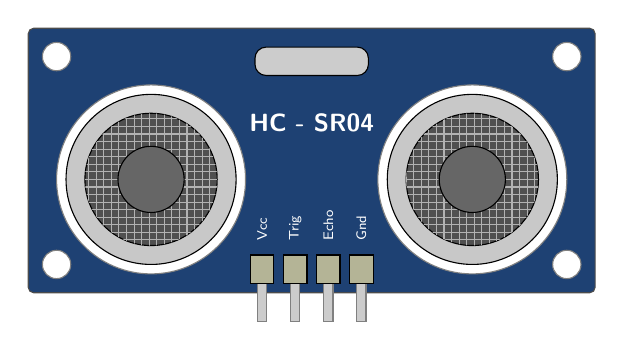
\begin{tikzpicture}[scale=1.2] % scale kann angepasst werden, um das Bild zu vergrößern/verkleinern
		
		% Hauptplatine (PCB)
		\draw[fill=pcbblue, rounded corners=2pt, draw=black!70] (0,0) rectangle (6, 2.8);
		
		% Befestigungslöcher in den Ecken
		\foreach \x/\y in {0.3/0.3, 5.7/0.3, 0.3/2.5, 5.7/2.5} {
			\draw[fill=white, draw=gray] (\x, \y) circle (0.15);
		}
		
		% Quarz (Das silberne ovale Bauteil oben mittig)
		\draw[fill=gray!40, rounded corners=4pt] (2.4, 2.3) rectangle (3.6, 2.6);
		
		% Produktname
		\node[text=white, font=\sffamily\bfseries\small] at (3, 1.8) {HC - SR04};
		
		% Die beiden Ultraschallwandler (Sender & Empfänger)
		\foreach \xpos in {1.3, 4.7} {
			% Äußerer Ring
			\draw[fill=white, draw=gray] (\xpos, 1.2) circle (1.0);
			% Metallgehäuse
			\draw[fill=sensorbody] (\xpos, 1.2) circle (0.9);
			% Gitterstruktur Bereich
			\draw[fill=sensorinner] (\xpos, 1.2) circle (0.7);
			
			% Gitter-Muster
			\begin{scope}
				\clip (\xpos, 1.2) circle (0.7);
				\draw[step=0.08, black!30, thin] (\xpos-0.7, 1.2-0.7) grid (\xpos+0.7, 1.2+0.7);
			\end{scope}
			
			% Innerster Kreis (Wandler-Element)
			\draw[fill=black!60] (\xpos, 1.2) circle (0.35);
		}
		
		% Pins und Beschriftung unten
		\foreach \i/\txt in {0/Vcc, 1/Trig, 2/Echo, 3/Gnd} {
			% OPTIONAL: Die grauen Metall-Pins, die unten aus dem Board herausragen
			\draw[fill=gray!40, draw=black!50] (2.425 + \i*0.35, 0.1) rectangle (2.525 + \i*0.35, -0.3);
			
			% Pin-Lötstelle (kleine Quadrate, exakt mittig zentriert)
			\draw[fill=pincolor] (2.35 + \i*0.35, 0.1) rectangle (2.60 + \i*0.35, 0.4);
			
			% Beschriftung (vertikal, exakt mittig über den Pads)
			\node[text=white, font=\sffamily\tiny, rotate=90, anchor=west] at (2.475 + \i*0.35, 0.45) {\txt};
		}
		
	\end{tikzpicture}
	\caption{Schematische Darstellung des Ultraschallsensors HC-SR04}
	\label{fig:hcsr04_tikz}
\end{figure}

	Die elektrischen und physikalischen Parameter entstammen den offiziellen Spezifikationen von KT-elektronic \cite{KT:2012}.
	\begin{itemize}
		\item Betriebsspannung (VCC: +5 V DC $\pm 10\%$)
		\item Stromaufnahme: < 2 mA
		\item Messbare Distanz: 2 cm bis ca. 300 cm 
		\item Messauflösung: 3 mm
		\item Messintervall: 20 ms (maximal 50 Messungen pro Sekunde)
		\item Messwinkel: Bis zu $45^\circ$ bei kurzen Distanzen (< 1 m), Sendekegel von $15^\circ$ bei maximaler Distanz
		\item Abmessungen (L x B x T): 45 x 21 x 18 mm
	\end{itemize}



\paragraph{Schaltplan}
Das Modul besitzt vier Pins \ref{fig:hcsr04_tikz}. Der VCC-Pin ist mit der 5V-Spannungsversorgung des Mikrocontrollers verbunden, der GND-Pin (Pin 4) mit dem GND-Pin des Mikrocontrollers. Der TRIG-Eingang (Pin 2) und der ECHO-Ausgang (Pin 3) arbeiten mit TTL-Pegel. 
Hinweis bei 3.3V-Mikrocontrollern: Da der ECHO-Pin ein 5V-Signal liefert, muss dieser zwingend durch einen Spannungsteiler an den 3.3V-Eingang des Mikrocontrollers angepasst werden \cite{KT:2012}.

\section{Bibliothek}

\subsection{Beschreibung}                                                                                                 
Für die Ansteuerung des Sensors wird die externe C++ Bibliothek \textbf{NewPing} von Tim Eckel verwendet \cite{Eckel:2023}.

\subsection{Installation}                                                                                            
Die Bibliothek kann direkt über den internen Bibliotheksverwalter der Arduino IDE installiert werden \cite{Eckel:2023}.
\begin{itemize}                                                                                                                                                                                   
	\item \textbf{Data types:} Messzeiten in Mikrosekunden und Distanzen in Zentimetern werden als \PYTHON{unsigned int} deklariert, um Speicherplatz zu sparen und negative Distanzen auszuschließen.
	\item \textbf{Data structure:} Der Sensor wird als Objekt der Klasse \PYTHON{NewPing} instanziiert.                                                                                                                                                            
	\item \textbf{Data quantity:} Das Softwaredesign ist ressourcenschonend konzipiert. Es können bis zu 15 Ultraschallsensoren gleichzeitig und asynchron über ein einziges Board betrieben werden, bei einer Abtastrate von bis zu 30 Pings pro Sekunde je Sensor.
	\item \textbf{Data quality:} Die Bibliothek bietet integrierte digitale Filter. Die Funktion \PYTHON{pingmedian} verarbeitet mehrere Messwerte zu einem Median, was Rauschen und fehlerhafte Echos effektiv aus dem Datensatz entfernt.
\end{itemize}

\subsection{Funktionen}                                                          
Die wichtigsten Befehle der NewPing-Bibliothek umfassen \cite{Eckel:2023}:
\begin{itemize}
	\item \PYTHON{NewPing sonar}(TRIGGER\_PIN, ECHO\_PIN, MAX\_DISTANCE \refeq{fig:hcsr04_tikz}): Konstruktor zur Erstellung des Sensor-Objekts.
	\begin{itemize}
		\item \textbf {TRIGGER\_PIN (Der Auslöser):} 
		Dieser Anschluss entspricht Pin 2 auf dem HC-SR04 Modul und arbeitet mit einem regulären TTL-Pegel \cite{KT:2012}. Um einen neuen Messzyklus auszulösen, muss an diesem Triggereingang ein Signal mit einer fallenden Flanke für mindestens 10 \textmu s anliegen \cite{KT:2012}. Als direkte Reaktion auf dieses Signal sendet das Modul selbstständig ein 40 kHz Burst-Signal aus \cite{KT:2012}. In dem vorliegenden Code-Beispiel wird dieser Anschluss dem digitalen Pin 12 des Arduino zugewiesen.
		
		\item \textbf{ECHO\_PIN (Der Empfänger):} 
		Dieser Ausgang liegt auf Pin 3 des Sensormoduls und gibt das eigentliche Messergebnis ebenfalls als TTL-Pegel aus \cite{KT:2012}. Unmittelbar nach dem Aussenden des Ultraschall-Bursts springt dieser Pin auf einen HIGH-Pegel und wartet auf den Empfang des zurückkehrenden Echos \cite{KT:2012}. Sobald das reflektierte Signal detektiert wird, fällt der Ausgang sofort auf einen LOW-Pegel ab \cite{KT:2012}. Wird gar kein Echo erkannt (weil der Raum leer ist), verweilt der Pin für exakt 200 ms auf dem HIGH-Pegel, um dem Mikrocontroller die erfolglose Messung zu signalisieren \cite{KT:2012}. In der Software ist dieser Pin dem digitalen Pin 11 zugewiesen.
		
		\item \textbf{MAX\_DISTANCE (Die maximale Reichweite):} 
		Rein physikalisch besitzt der HC-SR04 eine messbare Distanz von 2 cm bis zu ca. 300 cm \cite{KT:2012}. Soll die maximale Distanz von 3 Metern erreicht werden, muss der Sensor sehr exakt auf das Objekt zielen, und es dürfen keine störenden Gegenstände im Sendekegel von $15^\circ$ vorhanden sein \cite{KT:2012}. Im Programmcode ist \python{MAX\_DISTANCE} eine festgelegte Konstante (hier auf 200 cm gesetzt), die dem \python{NewPing}-Objekt mitteilt, bis zu welcher Entfernung der Sensor überhaupt auf Objekte reagieren soll \cite{Eckel:2023}.
	\end{itemize}
	\item\PYTHON{sonar.ping()}: Sendet einen Ping und gibt die gemessene Laufzeit in Mikrosekunden (\textmu s) zurück.
	\item \PYTHON{sonar.ping\_cm()}: Führt eine Messung durch und gibt die in Zentimeter (cm) umgerechnete Distanz zurück.
	\item \PYTHON{sonar.ping\_median(int iterations)}: Führt die angegebene Anzahl an Pings durch, verwirft Ausrei\ss er und gibt die mediane Laufzeit zurück.
\end{itemize}

\section{Beispiel}
In diesem Abschnitt wird ein einfaches, eigenständiges Codebeispiel beschrieben, welches die Funktionsweise und Integration der Bibliothek in C++ verdeutlicht.

\subsection{Handbuch}

\begin{enumerate}
	\item Verbinden Sie VCC und GND des HC-SR04 mit 5V und GND des Boards \cite{KT:2012}. 
	\item Verbinden Sie den TRIG-Pin mit Pin 12 und den ECHO-Pin mit Pin 11.
	\item Öffnen Sie die Arduino IDE, kompilieren Sie den Code und laden Sie ihn hoch.
	\item Öffnen Sie den Seriellen Monitor (Baudrate 115200). Hier werden nun die Messergebnisse ausgegeben\cite{SparkFun:2020}.
\end{enumerate} 

\subsection{Funktion vom Beispiel}                                                                                                                                                                                                                                                                                                                                                                                                                                      
Das Skript bindet die \PYTHON{NewPing.h} ein. Über \PYTHON{\#define} werden Pins und der maximale Messbereich (200 cm) definiert. In der Hauptschleife (\PYTHON{loop()}) stellt \PYTHON{delay(50)} sicher, dass zwischen zwei Pings gewartet wird, um Echosüberlappungen zu verhindern \cite{Eckel:2023}. Anschlie\ss end wird \PYTHON{ping\_median(5)} aufgerufen. Ist ein Objekt vorhanden, muss die gemessene Zeit in eine Längeneinheit umgewandelt werden. Hierfür kommt der bibliotheksinterne Befehl \PYTHON{US\_ROUNDTRIP\_CM} zum Einsatz. Dies ist eine vordefinierter Teilerfaktor, mit dem Wert 57. Er basiert auf der physikalischen Schallgeschwindigkeit in der Luft. Da der Schall für einen Zentimeter Wegstrecke etwa 29 Mikrosekunden benötigt und das Signal den Weg doppelt zurücklegen muss (Hin- und Rückweg), entspricht 1 cm Objektabstand exakt einer Signallaufzeit von ca. 57 bis 58 Mikrosekunden. Durch die Division \PYTHON{uS / US\_ROUNDTRIP\_CM} wird die gemessene Zeit somit effizient und direkt in den korrekten Zentimeter-Abstand umgerechnet \cite{Eckel:2023}.

\subsection{Code}

\begin{center}
	\captionof{code}{Beispiel Code} \label{code:Beispiel} \ArduinoExternal{}{../../Code/Ultraschallsensor/Beispielcode/Beispielcode.ino} 
\end{center}

%\subsection{Dateien}

\section{Kalibrierung}
Die Ultraschallmessung beruht auf der Ausbreitungsgeschwindigkeit von Schall in der Luft. Um das System zu überprüfen wird ein Objekt in einem exakt gemessenem Abstand vor dem Sensor aufgestellt und mit der Ausgabe im seriellen Monitor verglichen. Die Standardberechnung der Bibliothek geht von einer konstanten Schallgeschwindigkeit von $c \approx 343 \, \text{m/s}$ bei $20\,^\circ\text{C}$ aus \cite{Fraden:2016} . Da die Schallgeschwindigkeit temperaturabhängig ist, ändert sie sich um ca. $0,6 \, \text{m/s}$ pro Grad Celsius \cite{Fraden:2016}. Für hochpräzise Anwendungen muss das System kalibriert werden (z.B. über einen DHT22-Sensor). Die dynamische Berechnung lautet:
\[ \text{Distanz} = \frac{\text{Laufzeit}}{2} \times \left(331,3 + 0,606 \times \text{Temperatur in } ^\circ\text{C}\right) \].

\section{Einfacher Code ohne newPing Bibliothek}
Der folgende Code demonstriert eine Abstandsmessung ohne Einbindung der \python{NewPing}-Bibliothek und nutzt \python{pulseIn()}.

\begin{center}
	\captionof{code}{Beispiel Code ohne Bibliothekseinbindung} 
	\label{code: Beispiel2} \ArduinoExternal{}{../../Code/Ultraschallsensor/Beispielcode2/Beispielcode2.ino} 
\end{center}

\section{Einfache Anwendung}                                                                                                                  
Eine anschauliche Anwendung für den HC-SR04 ist eine automatisierte Einparkhilfe. Fährt ein Fahrzeug heran, liest der Sensor die Distanz. Unterschreitet der \python{distance}-Wert 50 cm, schaltet das System eine Warn-LED ein. Fällt der Wert auf unter 10 cm, wird ein Buzzer getriggert \cite{Eckel:2023}.

\begin{center}
	\captionof{code}{Einparkhilfe Beispielcode} \label{code:Einparkhilfe} \ArduinoExternal{}{../../Code/Ultraschallsensor/EinparkhilfeCode/EinparkhilfeCode.ino} 
\end{center}
\section{Tests}

\subsection{Einfacher Funktionstest}
Für die Überprüfung der grundlegenden Schaltung und Sensorik wird das Standalone-Skript aus Abschnitt \ref{code:Beispiel} (Gefilterte Distanzmessung mit der NewPing-Bibliothek) auf den Mikrocontroller geladen. 

Ein harter, planer Gegenstand (z.\,B. ein Buch) wird in exakt 15 cm Entfernung parallel zur Sensorfront platziert. Anschlie\ss end wird der Serielle Monitor der Arduino IDE mit einer Baudrate von 115200 geöffnet. 
Der ausgegebene Wert muss durch den Aufruf der Funktion \PYTHON{sonar.ping\_median(5)} sehr stabil bei 15 cm liegen. Die Schwankung darf dabei die gerätespezifische Auflösung des Moduls von 3 mm \cite{KT:2012} kaum überschreiten. Das Skript bestätigt somit, dass das Sende- und Empfangsmodul korrekt arbeiten und die serielle Datenübertragung fehlerfrei funktioniert.

\subsection{Alle Funktionen testen}
Ein vollständiger Systemtest kann wie folgt durchgeführt werden. Hierfür können die Ausgaben des Seriellen Monitors aus dem vorherigen Testcode \ref{code:Beispiel} oder das Verhalten der LEDs aus dem Parkassistenten-Code \ref{code:Einparkhilfe}  beobachtet werden:

\begin{itemize}
	\item \textbf{Minimaldistanz:} Das Objekt wird auf unter 2 cm an den Sensor herangeführt. Da der Sensor nach dem Senden des 200 \textmu s langen Bursts eine kurze Umschaltzeit benötigt \cite{KT:2012}, kann er Echos im absoluten Nahbereich physikalisch nicht mehr auflösen. Der Monitor sollte hier durch die Bibliothek korrekterweise Au\ss erhalb der Reichweite (Rückgabewert 0) ausgeben \cite{Eckel:2023}.
	
	\item \textbf{Maximaldistanz:} Der Sensor wird in einen leeren, gro\ss en Raum gerichtet, sodass das nächste Hindernis mehr als 300 cm entfernt ist. Laut Spezifikation verweilt der ECHO-Pin bei einem fehlenden Echo für 200 ms auf einem HIGH-Pegel \cite{KT:2012}. Der Test belegt, dass die NewPing-Bibliothek diesen Hardware-Timeout sicher abfängt, ohne dass sich der Mikrocontroller in einer blockierenden Endlosschleife aufhängt \cite{Eckel:2023}.
	
	\item \textbf{Winkeltest (Abstrahlkegel):} Ein Objekt wird in 50 cm Entfernung positioniert und langsam seitlich aus dem Zentrum bewegt. Überschreitet der Winkel $15^\circ$ zur Mittelachse, wird die Fläche vom Objekt für die Ultraschallwellen zu klein \cite{KT:2012}. Die Messwerte brechen ab, was die seitlichen Grenzen des Erfassungsbereichs bestätigt.
	
	\item \textbf{Dynamischer Reaktionstest:} Mit dem Code des automatisierten Parkassistenten aus Abschnitt \ref{code:Einparkhilfe} wird die Reaktionsgeschwindigkeit der Gesamtanlage getestet. Ein Objekt wird zügig auf den Sensor zubewegt. Die gelbe Warn-LED muss exakt beim Unterschreiten der 50-cm-Marke aufleuchten, und der Buzzer muss ohne spürbare Software-Verzögerung bei exakt 10 cm triggern.
\end{itemize}

\section{Weiterführende Literatur}

SparkFun Electronics / ElecFreaks (2019): HC-SR04 Ultrasonic Sensor Datasheet, Verfügbar unter: \url{https://www.sparkfun.com/datasheets/Sensors/Ultrasonic/HCSR04.pdf} [abgerufen am 28.04.2026]

\begin{itemize}
	\item Diese technische Spezifikation bildet die fundamentale Grundlage für die Ansteuerung. Sie enthält die exakten Timing-Diagramme für das Trigger- und Echo-Signal sowie Angaben zum Öffnungswinkel des Schallkegels, die für die Gehäuseplanung wichtig sind.
\end{itemize}

Eckel, Tim (2023): Arduino NewPing Library Documentation, GitHub/Bitbucket Repository, Verfügbar unter: \url{https://bitbucket.org/teckel12/arduino-newping/wiki/Home} [abgerufen am 28.04.2026]

\begin{itemize}
	\item Eine umfassende Dokumentation zur verwendeten Programmbibliothek NewPing Library von Tim Eckel. Es werden die Vorteile gegenüber herkömmlichen Messmethoden erläutert und die Implementierung von Filtern wie der \texttt{ping\_median()}-Funktion zur Rauschunterdrückung detailliert beschrieben.
\end{itemize}

Ekbert Hering und Gert Schönfelder, Sensoren in Wissenschaft und Technik – Funktionsweise und Einsatzgebiete, Springer Vieweg, 2023, ISBN: 9783658394905 \cite{Ekbert:2023}

\begin{itemize}
	\item Eine umfassende und aktuelle Einführung in die Grundlagen und Anwendungen von Sensoren in Technik, Biologie und Medizin. Das Buch behandelt neben physikalischen Grundlagen auch Themen wie Schnittstellen, Sicherheit und Signalverarbeitung bei Ultraschallwandlern.
\end{itemize}
